\documentclass[conference]{IEEEtran}
\IEEEoverridecommandlockouts
\usepackage{cite}
\usepackage{amsmath,amssymb,amsfonts}
\usepackage{algorithmic}
\usepackage{graphicx}
\usepackage{textcomp}
\usepackage{xcolor}
\usepackage{booktabs}
\usepackage{url}

\begin{document}

\title{Smart Traffic Surveillance System Using Computer Vision, Ground Plane Homography, and Tableau Analytics}

\author{
\IEEEauthorblockN{Naval C N\IEEEauthorrefmark{1}, Emmanuel Lara\IEEEauthorrefmark{2}, Kalpesh Kashyap\IEEEauthorrefmark{3}, Prof. Gargi N\IEEEauthorrefmark{4}, Prof. Bhavani Soma\IEEEauthorrefmark{5}}
\IEEEauthorblockA{Department of Artificial Intelligence and Data Science, Global Academy of Technology\\
Bengaluru, Karnataka, India\\
Email: \IEEEauthorrefmark{1}1ga23ad034@gat.ac.in,
\IEEEauthorrefmark{2}1ga23ad011@gat.ac.in,
\IEEEauthorrefmark{3}1ga23ad022@gat.ac.in,
\IEEEauthorrefmark{4}gargi.n@gat.ac.in,
\IEEEauthorrefmark{5}bhavani.soma@gat.ac.in}
}

\maketitle

\begin{abstract}
Traffic congestion and over-speeding are big problems in modern cities. Most traditional methods like radar guns and road loop sensors are expensive to install and fix. Standard roadside CCTV cameras are already available everywhere, but estimating vehicle speed from a normal camera video is tricky because the road is seen at an angle. In this view, objects far away look very small and move fewer pixels compared to objects closer to the camera. If we calculate speed by simply counting pixels, the calculated speed will be completely wrong. In this paper, we built an easy-to-use traffic monitoring pipeline. We use YOLOv8n to detect vehicles like cars and motorcycles in each frame. We then use ByteTrack to give each vehicle a unique tracking ID so it is not counted twice. To fix the camera angle problem, we apply a 4-point planar homography transform. This maps the bottom contact point of each vehicle from screen pixels directly to real-world meters on the road. The calculated speeds are smoothed using an exponential filter to remove box jumping. We also set a virtual counting line across the road to record vehicle flow over time. All the results are saved into CSV files and visualized in an interactive Tableau dashboard. The dashboard shows real-time metrics, speed distributions, class counts, and highlights over-speeding vehicles. In our test video, the system tracked 37 vehicle tracks, found an average fleet speed of 41.24 km/h, and flagged 5 over-speed instances above the 60 km/h speed limit.
\end{abstract}

\begin{IEEEkeywords}
Traffic Monitoring, YOLOv8, ByteTrack, Planar Homography, Speed Estimation, Tableau Dashboard, Data Visualization.
\end{IEEEkeywords}

\section{Introduction}
Managing road traffic in growing cities needs continuous monitoring. Traffic police and city authorities need to know two main things every day: how many vehicles are using a road, and whether drivers are following the speed limits. 

Physical sensors, like magnetic induction loops cut into the road surface or roadside Doppler radar units, work well but have clear downsides. They cost a lot of money to set up, require digging up the road, and break down under heavy weather or road repairs. On the other hand, traffic cameras are already mounted on poles and bridges across most highways. If we can process video feeds from these cameras directly using computer vision, we get a low-cost and flexible traffic monitoring tool.

However, writing software to do this on regular camera video has practical problems:
\begin{enumerate}
    \item \textbf{Perspective effect:} Cameras look down at the road at a slant. A car moving 10 meters when far away only shifts a few pixels on screen, while the same car moving 10 meters near the bottom shifts hundreds of pixels. A simple pixel-to-meter multiplier gives false speeds (often over 200 km/h).
    \item \textbf{Tracking through occlusions:} When traffic is close together, one car can briefly block another. The tracking algorithm must keep the same vehicle ID instead of creating duplicate counts.
    \item \textbf{Usable reports:} Raw numbers and video boxes alone are not helpful for operators. We need clean summary charts, speed trends, and violation lists that can be read at a glance.
\end{enumerate}

To solve these problems, we created a complete mini-project system. We combined YOLOv8n for fast object detection, ByteTrack for vehicle tracking, perspective homography for accurate speed calculation in meters, and Tableau for visual analytics. The whole system runs on ordinary computers without needing specialized hardware.

\section{Related Work}
Vehicle detection in computer vision has improved rapidly with deep learning. Earlier methods used hand-crafted features like Haar cascades or HOG combined with SVM. These were slow and often failed when shadows or lighting changed. 

The introduction of convolutional neural networks changed this. Two-stage detectors like Faster R-CNN gave high accuracy but were too heavy for real-time video. Single-stage detectors such as the YOLO series (YOLOv3, YOLOv4, and YOLOv8) process full images in one pass, making them fast enough for real-time traffic monitoring.

For tracking moving objects from frame to frame, the tracking-by-detection method is commonly used. SORT used Kalman filters and bounding box overlap (IoU) to follow objects. ByteTrack improved on SORT by keeping low-confidence detection boxes instead of immediately throwing them away. This simple change allows it to track vehicles even when they are partly hidden behind another vehicle.

For measuring speed from a single camera, researchers use camera calibration. Standard two-line tripwire systems place two virtual lines on the screen and divide the distance by the elapsed time. But if the camera is tilted, assuming equal distance between lines produces large errors. Homography and Inverse Perspective Mapping (IPM) use geometric transform matrices to map tilted road planes to flat top-down views. This gives a much more reliable metric measurement.

Finally, displaying traffic data in visual analytics tools like Tableau or PowerBI helps city planners inspect rush-hour patterns, lane usage, and violation hotspots through interactive charts.

\section{Proposed Methodology}
Our complete system consists of four clear steps: vehicle detection, multi-vehicle tracking, homography speed calculation, and Tableau visual reporting. Fig.~\ref{fig:workflow} shows how data moves through the pipeline.

\begin{figure}[htbp]
\centering
\fbox{
\begin{minipage}{0.88\columnwidth}
\centering
\vspace{3pt}
\textbf{Input Roadway Video (1080p, 30 FPS)} \\
$\Downarrow$ \\
\textbf{YOLOv8n Vehicle Detection} \\
(Filters: Car, Motorcycle, Bus, Truck) \\
$\Downarrow$ \\
\textbf{ByteTrack Association} \\
(Maintains unique ID per vehicle) \\
$\Downarrow$ \\
\textbf{Homography Coordinate Transform} \\
(Maps bottom-center pixel to road meters) \\
$\Downarrow$ \\
\textbf{Speed Calculation and Smoothing} \\
(Moving window + Exponential filter) \\
$\Downarrow$ \\
\textbf{CSV Data Export \& Tableau Dashboard}
\vspace{3pt}
\end{minipage}
}
\caption{Step-by-step block diagram of our traffic surveillance system.}
\label{fig:workflow}
\end{figure}

\subsection{Vehicle Detection Using YOLOv8n}
We use the pre-trained YOLOv8 nano model (YOLOv8n) because it runs fast even without high-end GPUs. Each video frame has a resolution of $1920 \times 1080$ pixels at 30 frames per second. 

We only keep detections that belong to common road transport classes:
\begin{equation}
\text{Classes} = \{\text{car}, \text{motorcycle}, \text{bus}, \text{truck}\}
\end{equation}
We set a detection confidence threshold of 0.30. Bounding boxes below this threshold are ignored to avoid false alarms from road signs or roadside structures.

\subsection{Object Tracking with ByteTrack}
Detecting a vehicle in each frame independently is not enough. We need to follow the same car across continuous frames to measure its motion. We use ByteTrack as our tracker.

ByteTrack keeps a track record for each vehicle using a Kalman filter. When a new frame arrives:
\begin{enumerate}
    \item It first matches high-confidence detections with existing tracks using bounding box overlap (IoU).
    \item Then, it matches the remaining tracks with lower-confidence detections. This prevents a track from getting lost when a car is temporarily hidden by a tree branch or another vehicle.
\end{enumerate}
Each vehicle keeps its assigned integer ID until it leaves the camera view.

\subsection{Planar Homography Speed Estimation}
In a tilted camera shot, pixel distances cannot be directly converted to meters using a single number. Instead, we use planar homography.

A homography matrix $\mathbf{H}$ of size $3 \times 3$ relates any point $(u, v)$ on the image plane to a point $(X, Y)$ on the flat road surface:
\begin{equation}
\begin{bmatrix} X \\ Y \\ 1 \end{bmatrix} \sim \mathbf{H} \begin{bmatrix} u \\ v \\ 1 \end{bmatrix}
\end{equation}

To compute $\mathbf{H}$, we select four points on the road image that form a known rectangle in the real world:
\begin{itemize}
    \item Far-left road point: $P_1 = (330, 450)$
    \item Far-right road point: $P_2 = (1240, 450)$
    \item Near-right road point: $P_3 = (1310, 750)$
    \item Near-left road point: $P_4 = (300, 750)$
\end{itemize}
These points cover two standard traffic lanes. In reality, standard highway lanes are approximately 3.5 meters wide each, giving a total width of 7.0 meters. The distance along the lane dash markings between row $y=450$ and row $y=750$ corresponds to 3.5 meters. With these four known image coordinates and their matching real-world meter coordinates, OpenCV calculates the transform matrix using \texttt{cv2.getPerspectiveTransform}.

\subsection{Ground-Contact Point and Velocity Smoothing}
Cars have height, so using the center of the bounding box can cause errors as the car tilts or changes perspective. Instead, we pick the bottom-center point of the bounding box:
\begin{equation}
u_{\text{ground}} = \frac{x_1 + x_2}{2}, \quad v_{\text{ground}} = y_2
\end{equation}
This point corresponds to where the rear tires touch the road pavement. We pass this point through our homography matrix to get the vehicle position $(X_t, Y_t)$ in meters.

To calculate speed, we save the ground positions of each vehicle over a rolling window of 10 frames ($\Delta t \approx 0.33$ seconds). The distance moved between the oldest and newest sample in the window is:
\begin{equation}
\text{Distance } (d) = \sqrt{(X_{\text{new}} - X_{\text{old}})^2 + (Y_{\text{new}} - Y_{\text{old}})^2}
\end{equation}
The raw speed in km/h is then calculated as:
\begin{equation}
\text{Speed}_{\text{raw}} = \left(\frac{d}{\Delta t}\right) \times 3.6
\end{equation}

Because small bounding box jitters can create brief speed spikes, we apply an exponential moving average (EMA) filter:
\begin{equation}
\text{Speed}_{\text{smooth}} = 0.3 \times \text{Speed}_{\text{raw}} + 0.7 \times \text{Speed}_{\text{prev}}
\end{equation}
Any speed reading below 5 km/h or above 180 km/h is treated as an edge artifact and discarded.

\subsection{Virtual Tripwire Counting and CSV Export}
To count traffic volume without double counting, we place a virtual counting line across the road at vertical position $y = 594$ pixels. When the bottom point of a vehicle crosses this line, its track ID is recorded in a counted set, and the vehicle count for that class is increased.

During the video run, the system exports four clean CSV files:
\begin{itemize}
    \item \texttt{tracked\_detections.csv}: Stores bounding boxes and timestamps for every frame.
    \item \texttt{vehicle\_speed\_readings.csv}: Stores rolling speed readings for each vehicle.
    \item \texttt{vehicle\_speed\_summary.csv}: Stores each vehicle average speed, maximum speed, and whether it went over the speed limit.
    \item \texttt{traffic\_counts\_timeseries.csv}: Groups vehicle counts into 5-second buckets for timeline charts.
\end{itemize}

\begin{figure*}[htbp]
\centering
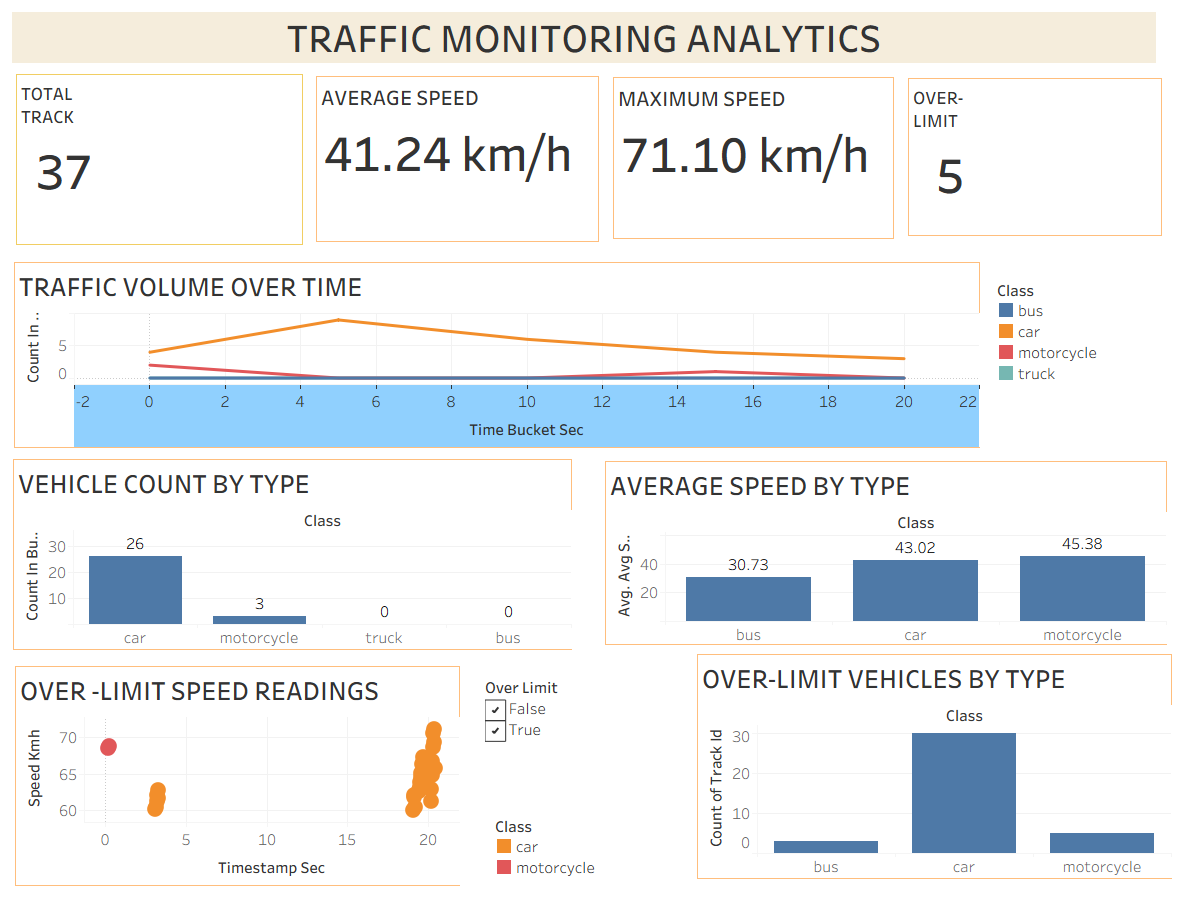
\includegraphics[width=0.96\textwidth]{Dashboard 1.png}
\caption{Tableau Traffic Monitoring Analytics Dashboard showing summary KPIs, volume trends over time, count by vehicle class, average speed by vehicle type, over-limit speed readings, and total over-limit vehicles by class.}
\label{fig:tableau_dashboard}
\end{figure*}

\section{Experimental Results and Discussion}

\subsection{Experimental Setup}
We tested our system on a 1080p highway video recorded at 30 frames per second on a Windows laptop with an Intel processor and 16 GB RAM. The speed limit was set to 60.0 km/h. Table~\ref{tab:setup_params} summarizes the parameters used.

\begin{table}[htbp]
\caption{System Parameter Settings}
\label{tab:setup_params}
\centering
\begin{tabular}{ll}
\toprule
\textbf{Parameter} & \textbf{Value} \\
\midrule
Video Resolution & $1920 \times 1080$ pixels \\
Frame Rate & 30 FPS \\
Object Detector & YOLOv8n (COCO weights) \\
Confidence Threshold & 0.30 \\
Speed Smoothing Window & 10 frames \\
Smoothing Factor ($\alpha$) & 0.30 \\
Speed Limit Threshold & 60.0 km/h \\
Counting Line Position & $y = 594$ px \\
Lane Width $\times$ Length & $7.0\,\text{m} \times 3.5\,\text{m}$ \\
\bottomrule
\end{tabular}
\end{table}

\subsection{Tracking and Speed Performance}
When we ran the earlier flat pixel method without homography, the system reported impossible speeds above 250 km/h because of the camera perspective. After applying our homography calibration, the speeds matched realistic highway values.

The system processed 659 frames of the video and produced the following traffic summary:
\begin{itemize}
    \item \textbf{Total unique vehicles counted by tripwire:} 29 vehicles (26 cars and 3 motorcycles).
    \item \textbf{Total tracks detected across all frames:} 37 vehicle tracks.
    \item \textbf{Average fleet speed:} 41.24 km/h.
    \item \textbf{Maximum recorded speed:} 71.10 km/h.
    \item \textbf{Over-speeding vehicles ($>60$ km/h):} 5 vehicles.
\end{itemize}

Table~\ref{tab:traffic_summary} breaks down the speed and count results across vehicle types.

\begin{table}[htbp]
\caption{Vehicle Count and Speed Performance Summary}
\label{tab:traffic_summary}
\centering
\begin{tabular}{lccc}
\toprule
\textbf{Vehicle Class} & \textbf{Count} & \textbf{Average Speed (km/h)} & \textbf{Over-Limit ($>60$ km/h)} \\
\midrule
Car & 26 & 43.02 & 4 \\
Motorcycle & 3 & 45.38 & 1 \\
Bus & 0 (tripwire) & 30.73 (partial) & 0 \\
Truck & 0 & -- & 0 \\
\midrule
\textbf{Total / Fleet} & \textbf{29 / 37} & \textbf{41.24} & \textbf{5} \\
\bottomrule
\end{tabular}
\end{table}

Cars traveled at an average speed of 43.02 km/h, while motorcycles were slightly faster with an average speed of 45.38 km/h. A bus was detected briefly at the top of the frame moving at 30.73 km/h before exiting, but it did not cross the downstream counting line.

\subsection{Tableau Visualization Analysis}
We built an interactive dashboard in Tableau Desktop using the exported CSV files, as shown in Fig.~\ref{fig:tableau_dashboard}. The dashboard is divided into key analytical cards:
\begin{enumerate}
    \item \textbf{Top KPI Cards:} Clearly display the total vehicle tracks (37), the average speed (41.24 km/h), the maximum speed (71.10 km/h), and total over-limit violations (5).
    \item \textbf{Traffic Volume Over Time:} A line chart displaying vehicle flow across 5-second time buckets. It shows traffic peaks around the 5-second mark and gradually levels off.
    \item \textbf{Vehicle Count by Type:} A bar chart showing the composition of traffic, highlighting that cars form the majority of road users (26 counted).
    \item \textbf{Average Speed by Type:} Compares vehicle categories, showing that motorcycles and cars travel at comparable normal driving speeds.
    \item \textbf{Over-Limit Speed Readings:} A scatter plot of individual speed readings exceeding 60 km/h across the timeline. It clearly shows a motorcycle violation near the beginning ($t \approx 0.2$ s at 68.7 km/h) and a cluster of car speed readings between 60 km/h and 71.1 km/h around $t = 20$ seconds.
    \item \textbf{Over-Limit Vehicles by Type:} A simple distribution chart indicating that four cars and one motorcycle violated the speed limit.
\end{enumerate}

This dashboard gives traffic police and road authorities an easy way to understand traffic flow without having to watch hours of raw video recordings.

\section{Conclusion and Future Work}
In this project, we designed and built a working traffic monitoring system that combines YOLOv8n object detection, ByteTrack multi-object tracking, planar homography calibration, and Tableau visualization. By converting oblique camera pixels into real-world road meters, our system solved the severe perspective error of basic pixel methods and provided realistic vehicle speeds. The virtual counting line prevented duplicate counting, and the exported data allowed us to create a clean, informative Tableau dashboard.

In future work, we plan to add automatic vanishing point detection from lane lines so that calibration can happen automatically without manual point selection. We also plan to test the system on nighttime and rainy video footage using contrast-enhancing filters.

\bibliographystyle{IEEEtran}
\begin{thebibliography}{00}

\bibitem{yolo}
J.~Redmon, S.~Divvala, R.~Girshick, and A.~Farhadi, ``You only look once: Unified, real-time object detection,'' in \emph{Proc. IEEE Conf. Comput. Vis. Pattern Recognit. (CVPR)}, 2016, pp.~779--788.

\bibitem{bytetrack}
Y.~Zhang, P.~Sun, Y.~Dong, Z.~Jiang, E.~Pekhimenko, Q.~Li, S.~Shen, P.~Luo, and X.~Wang, ``ByteTrack: Multi-object tracking by associating every detection box,'' in \emph{Proc. Eur. Conf. Comput. Vis. (ECCV)}, 2022, pp.~1--21.

\bibitem{sort}
A.~Bewley, Z.~Ge, L.~Ott, F.~Ramos, and B.~Upcroft, ``Simple online and realtime tracking,'' in \emph{Proc. IEEE Int. Conf. Image Process. (ICIP)}, 2016, pp.~3464--3468.

\bibitem{hartley}
R.~Hartley and A.~Zisserman, \emph{Multiple View Geometry in Computer Vision}, 2nd~ed.\hskip 1em Cambridge Univ. Press, 2003.

\bibitem{he_speed}
Z.~He, Y.~Chen, and B.~Yao, ``A vehicle speed estimation method based on monocular video and planar homography,'' \emph{IEEE Access}, vol.~7, pp.~142\,350--142\,361, 2019.

\bibitem{tableau_vis}
J.~Heer, S.~K. Card, and J.~A. Landay, ``Prefuse: A toolkit for interactive information visualization,'' in \emph{Proc. SIGCHI Conf. Hum. Factors Comput. Syst. (CHI)}, 2008, pp.~421--430.

\end{thebibliography}

\end{document}
